\documentclass{beamer}
\usepackage{../tut-slides}
\usepackage{../mathoperatorsAuD}

\usepackage{lmodern}
\usepackage{amsmath,amssymb}
\usepackage{wasysym}
\usepackage{stmaryrd}
\usepackage{enumerate}
%\usepackage[inline]{enumitem} 		%customize label
%\newcommand{\labelitemi}{\raisebox{1pt}{\scalebox{.9}{$\blacktriangleright$}}}
%\newcommand{\labelitemii}{$\vartriangleright$}
%\newcommand{\labelitemiii}{--}
\setbeamertemplate{itemize item}{\raisebox{1pt}{\scalebox{.9}{$\blacktriangleright$}}}
\setbeamertemplate{itemize subitem}{$\vartriangleright$}

\usepackage{booktabs}
\usepackage{tabularx}
\usepackage{tabu}
\newcommand*\head{\rowfont{\bfseries}}
\newcommand*{\tw}{\rowfont{\ttfamily}}
\renewcommand{\tabularxcolumn}[1]{>{\hspace{0pt}}m{#1}}
\usepackage{multirow}

\usepackage{cancel}

\usepackage{empheq}
\newcommand*\widefbox[1]{\fbox{\hspace{2em} #1 \hspace{2em}}}

\usepackage{tcolorbox}
\newtcolorbox{mymathbox}[1][]{colback=white, sharp corners, #1}

\usepackage{xcolor}
\usepackage{listings}
\lstset{numbers=left, 
	numberstyle=\tiny, 
	breaklines=true,
	backgroundcolor=\color{cdgray!20},
	numbersep=5pt,
	language=C,
	tabsize=2,
	basicstyle=\footnotesize\ttfamily,
	showstringspaces=false} 

\DeclareMathOperator{\ack}{\mathbf{ack}}
\usepackage{MnSymbol}

\newcommand{\col}[1]{\textcolor{cdpurple}{#1}}
\newcolumntype{R}[1]{>{\centering\arraybackslash}p{#1}}
\usepackage{tabularx}
\renewcommand{\tabularxcolumn}[1]{m{#1}}

\usepackage{qtree}
\usepackage[edges]{forest}

\newcommand{\lefttree}{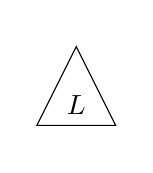
\begin{tikzpicture}
	\draw (0,0) node[anchor=north]{}
	-- (1,0) node[anchor=north]{}
	-- (.5,1) node[anchor=south]{}
	-- cycle;
	\draw (.5,.5) node[anchor=north]{$L$};
	\end{tikzpicture}}
\newcommand{\righttree}{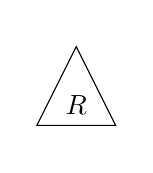
\begin{tikzpicture}
	\draw (0,0) node[anchor=north]{}
	-- (1,0) node[anchor=north]{}
	-- (.5,1) node[anchor=south]{}
	-- cycle;
	\draw (.5,.5) node[anchor=north]{$R$};
	\end{tikzpicture}}


\begin{document}	
	\title{Algorithmen und Datenstrukturen}
	\subtitle{Übung 10: Suchen \& Korrigieren, AVL-Bäume}
	\author{Eric Kunze}
	\email{eric.kunze@mailbox.tu-dresden.de}
	\city{TU Dresden}
%	\institute{Lehrstuhl für Grundlagen der Programmierung}
	\titlegraphic{
\includegraphics[width=2cm]{../TUD-white.pdf}}
	\date{09.01.2020}

	\maketitle


%%%%%%%%%%%%%%%%%%%%%%%%%%%%%%%%%%%%%%%%%%%%%%%%%%%%%%%%%%%%%%%%%%%%%%%%%%%%%

\begin{frame} \frametitle{Algorithmen und Datenstrukturen}
	\textbf{Was bisher geschah ...}
	\begin{itemize}
		\item Syntax von Programmiersprachen \\
		 (Syntaxdiagramme, EBNF, Fixpunktsemantik)
		\item Programmieren in $C$ -- Arrays, Pointer, Listen, Bäume
		\item grundlegende Algorithmen in der Informatik
		\begin{itemize}
			\item Sortieren mit Quicksort und Heapsort
			\item Suchen in Texten (KMP-Algorithmus)
		\end{itemize}		
	\end{itemize}

	\pause

	\textbf{Was heute geschieht ...}
	\begin{itemize}
		\item Wiederholung: Suche mit dem KMP-Algorithmus
		\item Fehlerkorrektur mit der Levenshtein-Distanz
		\item Balancieren von Bäumen (AVL-Bäume)
	\end{itemize}
\end{frame}


\section{KMP-Algorithmus} 

\begin{frame} \frametitle{KMP-Algorithmus --- Die Zwei-Finger-Methode}
	Die Methode beruht auf der Gleichung
	\begin{equation*}
		\begin{aligned}
		\small
		&\texttt{Tab[i]} \\
		= &\max \menge{-1} \cup \menge{m \mid 0 \le m \le i-1 \land b_0 \dots b_{m-i} = b_{i-m} \land b_{i-1} \land b_m \neq b_j}
		\end{aligned} \tag{$\star$} \label{eq: kmp}
	\end{equation*}
	Daraus ergibt sich nach Initialisierung von $\texttt{Tab[0]} = -1$ für jeden folgenden Eintrag $\texttt{Tab[i]}$ folgendes Verfahren:
	\begin{itemize}
		\item \textit{linker Finger}: wähle $m < i$ in absteigender Reihenfolge (also $i-1$, $i-2$, $\dots$), sodass $\texttt{Pat[i]} \neq \texttt{Pat[m]}$
		\item \textit{Parallelverschiebung beider Finger bis zum linken Rand}: wenn $\texttt{Pat[0 \dots m-1]} = \texttt{Pat[i-m \dots i-1]}$, dann fülle $\texttt{Tab[i]} = m$.
		\item wenn keine passende Position $m$ gefunden werden kann, dann fülle $\texttt{Tab[i]} = -1$.
	\end{itemize}
\end{frame}


\begin{frame} \frametitle{Aufgabe 1}
	\textbf{Teil (a)} \hspace{3em}
	Pattern: {\large \texttt{abbabbaa}} \\[1em]
	\pause
	
	\begin{center}
		\begin{tabular}{l|cccccccc}
			Position &  0 &  1 &  2 &  3 &  4 &  5 &  6 &  7  \\ \hline
			Pattern  &  a &  b &  b &  a &  b &  b &  a &  a  \\ \hline
			Tabelle  & -1 &  0 &  0 & -1 &  0 &  0 & -1 &  4  \\
		\end{tabular}
	\end{center}
	
	\pause

	\textbf{Teil (b)}
	\begin{center}
		\begin{tabular}{l|cccccc}
			Position &  0 &  1 &  2 &  3 &  4 &  5 \\ \hline
			Pattern  &  \textit{b} &  \onslide+<4->{a} &  \onslide+<4->{b} &  \onslide+<4->{a} &  \onslide+<4->{b} &  \textit{c} \\ \hline
			Tabelle  & -1 &  ? & ? &  0 &  ? &  3 \\
		\end{tabular}
	\end{center}

	\pause

	\footnotesize
	\begin{itemize}
		\item $\texttt{Pat[0 ... 2] = Pat[2 ... 4]}$ wegen $\texttt{Tab[5] = 3}$ (Zyklenmethode), d.h. $\texttt{Pat[2] = Pat[0] = Pat[4] = b}$
		\item wegen $\texttt{Tab[3] = 0}$ ist $\texttt{Pat[3]} \neq  \texttt{Pat[0] = b}$ und wegen $\texttt{Tab[5] = 3}$ ist $\texttt{Pat[3]} \neq \texttt{Pat[5] = c}$ (Zwei-Finger-Methode bzw. Gleichung \eqref{eq: kmp}) \\
		$\Rightarrow \texttt{Pat[3] = Pat[1] = a}$
	\end{itemize}
	
\end{frame}

%%%%%%%%%%%%%%%%%%%%%%%%%%%%%%%%%%%%%%%%%%%%%%%%%%%%%%%%%%%%%%%%%%%%%%%%%%%%%%%%%%%

\section{Levenshtein-Distanz}

\begin{frame} \frametitle{Levenshtein-Distanz}
	\textbf{Kosten} zur Überführung eines Wortes $w = w_1 \dots w_n$ in ein Wort $v = v_1 \dots v_k$ ; schreibe $d(w_1 \dots w_j, v_1 \dots v_i) = d(j,i)$.
	\pause
	\begin{align*}
		d(0,i) &= i \\
		d(j,0) &= j \\
		d(j,i) &= \min \menge{ d(j,i-1) + 1, d(j-1,i) + 1 , d(j-1, i-1) + \delta_{j,i}}
	\end{align*}
	für alle $1 \le j \le n$ und alle $1 \le i \le k$ wobei
	\begin{equation*}
		\delta_{j,i} = \begin{cases}
		1 & \text{wenn } w_j \neq v_i \\
		0 & \text{sonst}
		\end{cases} 
	\end{equation*}
	\pause
	\textbf{Anschaulich:} 
	Überlagerung durch Pattern
	$\to$ Pfeile zeigen ''Ursprung`` des Minimums an
	\begin{equation*}
		w_j \neq v_i : \quad \begin{array}{|c|c|}
			\hline +1 & +1 \\ \hline +1 & ? \\ \hline
		\end{array}
		\qquad \qquad
		w_j = v_i : \quad 
		\begin{array}{|c|c|}
		\hline +0 & +1 \\ \hline +1 & ? \\ \hline
		\end{array}
	\end{equation*}

\end{frame}
\begin{frame} \frametitle{Aufgabe 9.4}
		\centering
		\renewcommand*{\arraystretch}{.7}
		\setlength{\tabcolsep}{3pt}
			\begin{tabular}{l|ccccccccccccccc}
				$d(j,i)$ &       &       & \textbf{D} &       & \textbf{i} &       & \textbf{s} &       & \textbf{t} &       & \textbf{a} &       & \textbf{n} &       & \textbf{z} \\ \hline \\
				& 0     & $\rightarrow$ & 1     & $\rightarrow$ & 2     & $\rightarrow$ & 3     & $\rightarrow$ & 4     & $\rightarrow$ & 5     & $\rightarrow$ & 6     & $\rightarrow$ & 7 \\
				& $\downarrow$ & \alert<3->{$\searrow$} &       &       &       &       &       &       &       &       &       &       &       &       &  \\
				\textbf{D}     & 1     &       & 0     & $\rightarrow$ & 1     & $\rightarrow$ & 2     & $\rightarrow$ & 3     & $\rightarrow$ & 4     & $\rightarrow$ & 5     & $\rightarrow$ & 6 \\
				& $\downarrow$ &       & $\downarrow$ & \alert<3->{$\searrow$} &       &       &       &       &       &       &       &       &       &       &  \\
				\textbf{i}     & 2     &       & 1     &       & 0     & $\rightarrow$ & 1     & $\rightarrow$ & 2     & $\rightarrow$ & 3     & $\rightarrow$ & 4     & $\rightarrow$ & 5 \\
				& $\downarrow$ &       & $\downarrow$ &       & \alert<3->{$\downarrow$} & $\searrow$ &       & $\searrow$ &       & $\searrow$ &       & $\searrow$ &       &       &  \\
				\textbf{n}     & 3     &       & 2     &       & 1     &       & 1     & $\rightarrow$ & 2     & $\rightarrow$ & 3     &       & 3     & $\rightarrow$ & 4 \\
				& $\downarrow$ &       & $\downarrow$ &       & $\downarrow$ & \alert<3->{$\searrow$} &       & $\searrow$ &       & $\searrow$ &       & $\searrow$ & $\downarrow$ & $\searrow$ &  \\
				\textbf{s}     & 4     &       & 3     &       & 2     &       & 1     & $\rightarrow$ & 2     & $\rightarrow$ & 3     & $\rightarrow$ & 4     &       & 4 \\
				& $\downarrow$ &       & $\downarrow$ &       & $\downarrow$ &       & $\downarrow$ & \alert<3->{$\searrow$} &       &       &       &       &       &       &  \\
				\textbf{t}     & 5     &       & 4     &       & 3     &       & 2     &       & 1     & $\rightarrow$ & 2     & $\rightarrow$ & 3     & $\rightarrow$ & 4 \\
				& $\downarrow$ &       & $\downarrow$ &       & $\downarrow$ &       & $\downarrow$ &       & $\downarrow$ & \alert<3->{$\searrow$} &       &       &       &       &  \\
				\textbf{a}     & 6     &       & 5     &       & 4     &       & 3     &       & 2     &       & 1     & \alert<3-3>{$\rightarrow$} & 2     & $\rightarrow$ & 3 \\
				& $\downarrow$ &       & $\downarrow$ &       & $\downarrow$ & $\searrow$ & $\downarrow$ &       & $\downarrow$ &       & $\downarrow$ & \alert<4->{$\searrow$} &       & \alert<3-3>{$\searrow$} &  \\
				\textbf{s}     & 7     &       & 6     &       & 5     &       & 4     &       & 3     &       & 2     &       & 2     & \alert<4->{$\rightarrow$} & 3 \\
			\end{tabular}
		
		\pause
		\begin{equation*}
			d(\text{Dinstas}, \text{Distanz}) = 3
		\end{equation*}
\end{frame}

\begin{frame} \frametitle{Aufgabe 9.4}
	Alignments mit minimaler Levenshtein-Distanz:
	
	\centering
	
	\begin{tabular}{cccccccc}
		D & i & n & s & t & a & $\ast$ & s \\
		$|$ & $|$ & $|$ & $|$ & $|$ & $|$ & $|$ & $|$ \\
		D & i & $\ast$ & s & t & a & n & z \\
		  &   & \textit{d} &   &   &   & \textit{i} & \textit{s} \\
	\end{tabular}

	\vspace{3em}
	
	\begin{tabular}{cccccccc}
		D & i & n & s & t & a & s & $\ast$ \\
		$|$ & $|$ & $|$ & $|$ & $|$ & $|$ & $|$ & $|$ \\
		D & i & $\ast$ & s & t & a & n & z \\
		&   & \textit{d} &   &   &   & \textit{s} & \textit{i} \\
	\end{tabular}
\end{frame}

\begin{frame} \frametitle{Aufgabe 2}
	\centering
	\renewcommand*{\arraystretch}{.7}
	\setlength{\tabcolsep}{3pt}
	\begin{tabular}{l|rrrrrrrlrrrlrlr}
		$d(j,i)$ &       &       & \textbf{s} &       & \textbf{c} &       & \textbf{h} &       & \textbf{ü} &       & \textbf{r} &       & \textbf{z} &       & \textbf{e} \\ \hline \\
		& 0     & \alert<3->{$\rightarrow$} & 1     & \alert<3->{$\rightarrow$} & 2     & $\rightarrow$ & 3     & $\rightarrow$ & 4     & $\rightarrow$ & 5     & $\rightarrow$ & 6     & $\rightarrow$ & 7 \\
		& $\downarrow$ & \alert<4->{$\searrow$} &       & \alert<4->{$\searrow$} &       & \alert<3->{$\searrow$} &       & $\searrow$ &       & $\searrow$ &       & $\searrow$ &       & $\searrow$ &  \\
		\textbf{b}     & 1     &       & 1     & \alert<4->{$\rightarrow$} & 2     & \alert<4->{$\rightarrow$} & 3     & $\rightarrow$ & 4     & $\rightarrow$ & 5     & $\rightarrow$ & 6     & $\rightarrow$ & 7 \\
		& $\downarrow$ & $\searrow$ & $\downarrow$ & $\searrow$ &       & $\searrow$ &       & \alert<3->{$\searrow$} &       &       &       &       &       &       &  \\
		\textbf{ü}     & 2     &       & 2     &       & 2     & $\rightarrow$ & 3     &       & 3     & $\rightarrow$ & 4     & $\rightarrow$ & 5     & $\rightarrow$ & 6 \\
		& $\downarrow$ & $\searrow$ & $\downarrow$ & $\searrow$ & $\downarrow$ & $\searrow$ &       & $\searrow$ & $\downarrow$ & \alert<3->{$\searrow$} &       &       &       &       &  \\
		\textbf{r}     & 3     &       & 3     &       & 3     &       & 3     & $\rightarrow$ & 4     &       & 3     & $\rightarrow$ & 4     & $\rightarrow$ & 5 \\
		& $\downarrow$ & $\searrow$ &       & $\searrow$ & $\downarrow$ & $\searrow$ & $\downarrow$ & $\searrow$ &       &       & \alert<4->{$\downarrow$} & \alert<3->{$\searrow$} &       & $\searrow$ &  \\
		\textbf{s}     & 4     &       & 3     & $\rightarrow$ & 4     &       & 4     &       & 4     &       & 4     &       & 4     & $\rightarrow$ & 5 \\
		& $\downarrow$ &       & $\downarrow$ & $\searrow$ &       & $\searrow$ & $\downarrow$ & $\searrow$ & $\downarrow$ & $\searrow$ & $\downarrow$ & \alert<4->{$\searrow$} & \alert<3->{$\downarrow$} & $\searrow$ &  \\
		\textbf{t}     & 5     &       & 4     &       & 4     & $\rightarrow$ & 5     &       & 5     &       & 5     &       & 5     &       & 5 \\
		& $\downarrow$ &       & $\downarrow$ & $\searrow$ & $\downarrow$ & $\searrow$ &       & $\searrow$ & $\downarrow$ & $\searrow$ & $\downarrow$ & $\searrow$ & $\downarrow$ & \alert<3->{$\searrow$} &  \\
		\textbf{e}     & 6     &       & 5     &       & 5     &       & 5     & $\rightarrow$ & 6     &       & 6     & & 6     &  & 5 \\
	\end{tabular}%

	\pause

	\begin{equation*}
		d(\text{bürste}, \text{schürze}) = 5 \qquad \pause \pause \pause \text{Anzahl der Backtraces } = 3 * 2 = 6
	\end{equation*}
\end{frame}

\begin{frame} \frametitle{Aufgabe 2 --- Teil (b)}
	Alignments mit minimaler Levenshtein-Distanz zwischen den Wörtern
	\texttt{bürst} und \texttt{sch}
	
	\centering
	\renewcommand*{\arraystretch}{.7}
	\setlength{\tabcolsep}{3pt}
	\begin{tabular}{l|ccccccc}
		$d(j,i)$ &       &       & \textbf{s} &       & \textbf{c} &       & \textbf{h}  \\ \hline \\
		& 0     & $\rightarrow$ & 1     & $\rightarrow$ & 2     & $\rightarrow$ & 3  \\
		& \alert<2->{$\downarrow$} & \alert<2->{$\searrow$} &       & $\searrow$ &       & $\searrow$ &  \\
		\textbf{b}     & 1     &       & 1     & $\rightarrow$ & 2     & $\rightarrow$ & 3  \\
		& \alert<2->{$\downarrow$} & \alert<2->{$\searrow$} & \alert<2->{$\downarrow$} & \alert<2->{$\searrow$} &       & $\searrow$ &   \\
		\textbf{ü}     & 2     &       & 2     &       & 2     & $\rightarrow$ & 3  \\
		& \alert<2->{$\downarrow$} & \alert<2->{$\searrow$} & \alert<2->{$\downarrow$} & \alert<2->{$\searrow$} & \alert<2->{$\downarrow$} & \alert<2->{$\searrow$} & \\
		\textbf{r}     & 3     &       & 3     &       & 3     &       & 3 \\
		& $\downarrow$ & \alert<2->{$\searrow$} &       & \alert<2->{$\searrow$} & \alert<2->{$\downarrow$} & \alert<2->{$\searrow$} & \alert<2->{$\downarrow$}  \\
		\textbf{s}     & 4     &       & 3     & \alert<2->{$\rightarrow$} & 4     &       & 4  \\
		& $\downarrow$ &       & $\downarrow$ & \alert<2->{$\searrow$} &       & \alert<2->{$\searrow$} & \alert<2->{$\downarrow$} \\
		\textbf{t}     & 5     &       & 4     &       & 4     & \alert<2->{$\rightarrow$} & 5   \\
	\end{tabular}%
\end{frame}

\begin{frame} \frametitle{Aufgabe 2 --- Teil (b)}
	Alignments mit minimaler Levenshtein-Distanz zwischen den Wörtern
	\texttt{bürst} und \texttt{sch}
	
	\centering
	\begin{tabular}{ccccc}
		b & ü & r & s & t \\
		$|$ & $|$ & $|$ & $|$ & $|$ \\
		s & c & h & $\ast$ & $\ast$ \\
		\textit{s} & \textit{s} & \textit{s} & \textit{d} & \textit{d}  \\
	\end{tabular}
	\hspace{2em}
	\begin{tabular}{ccccc}
		b & ü & r & s & t \\
		$|$ & $|$ & $|$ & $|$ & $|$ \\
		$\ast$ & $\ast$ & s & c & h \\
		\textit{d} & \textit{d} & \textit{s} & \textit{s} & \textit{s}  \\
	\end{tabular}
\end{frame}

%%%%%%%%%%%%%%%%%%%%%%%%%%%%%%%%%%%%%%%%%%%%%%%%%%%%%%%%%%%%%%%%%%%%%%%%%%%%%%%%%%%

\section{AVL-Bäume}

\begin{frame} \frametitle{AVL-Bäume}
	Wir betrachten einen Baum $t$ und bezeichnen die \textit{Schlüssel} an den Knoten $n$ mit $s(n)$. 
	\pause
	
	\textbf{Suchbaum:} \Tree [.$s(n)$ [ .{\lefttree} ] [ .{\righttree} ] ] mit $L < s(n) < R$
	
	\pause
	
	Die \textit{Höhe} des Baumes bezeichnen wir mit $h(t)$.
	Wir ordnen jedem Knoten $n$ einen \textit{Balancefaktor} $b(n)$ zu:
	\begin{equation*}
		b(n) \defeq h(R) - h(L)
	\end{equation*}
	
	\pause
	\textbf{AVL-Baum:} Suchbaum mit $b(n) \in \menge{-1, 0, 1}$
\end{frame}

\begin{frame} \frametitle{Balancieren}
	\begin{itemize}
		\item Einfügen eines neuen Schlüssels $s$
		\item Berechne Balancefaktoren auf dem Pfad von $s$ zur Wurzel bis zum ersten Auftreten von $\pm 2$
		\item \textbf{Balancierungsalgorithmus}: 
		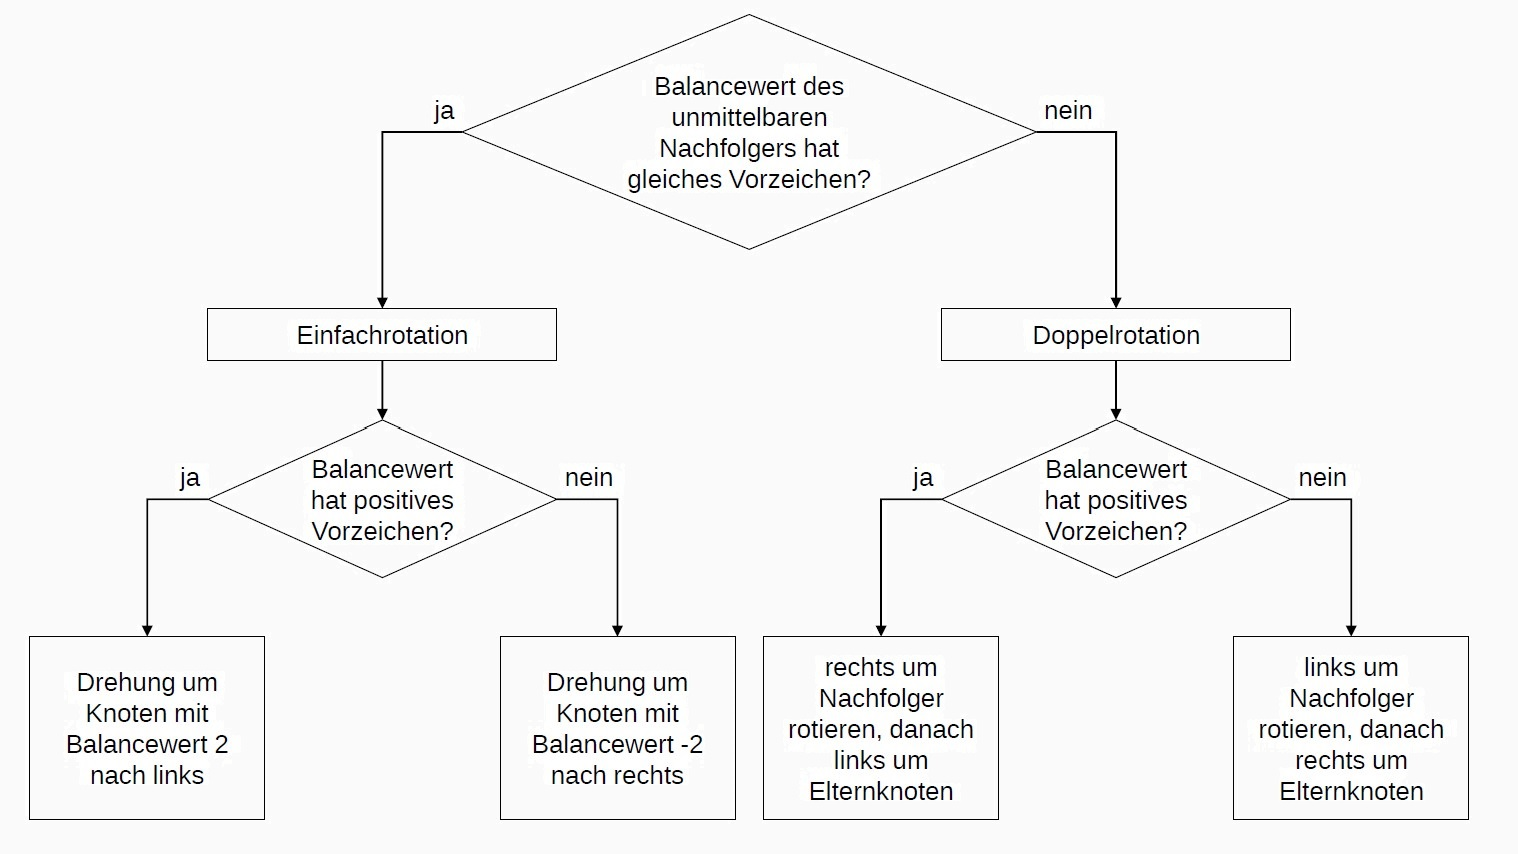
\includegraphics[width=\linewidth]{./tut10_avl.jpg}
	\end{itemize}
\end{frame}

\begin{frame} \frametitle{Aufgabe 3}
	\begin{tabularx}{\linewidth}{m{2cm} m{.8cm} m{2cm} m{.8cm} m{2cm}}
		\begin{forest}
			[ $2$ [ $1$ ] [$3$ [,no edge, draw=none] [ $4$ ]  ] ] 
		\end{forest} 
		&
		$\overset{i(5)}{\longrightarrow}$
		&
		\begin{forest}
			[ $2^2$ [ $1$ ] [ $3^2$ [,no edge, draw=none] [ $4^1$ [,no edge, draw=none] [ $5^0$ ]  ] ]  ]
		\end{forest}  
		&
		$\overset{L(3)}{\longrightarrow}$
		&
		\begin{forest}
			[ $2$ [ $1$ ] [ $4$ [ $3$ ] [ $5$ ] ] ]
		\end{forest}
	\end{tabularx}
\end{frame}

\begin{frame} \frametitle{Aufgabe 3}
	\centering
	\begin{tabularx}{\linewidth}{m{2cm} m{.8cm} m{4cm}}
		\begin{forest}
			[ $4$ [ $2$ [,no edge, draw=none] [ $3$ ]  ] [ $5$ ] ]
		\end{forest}
		&
		$\overset{i(1)}{\longrightarrow}$
		&
		\begin{forest}
			[ $4^{-1}$ [ $2^0$ [ $1^0$ ] [ $3$ ]  ] [ $5$ ] ]
		\end{forest} 
	\end{tabularx}
\end{frame}

\begin{frame} \frametitle{Aufgabe 3}
	\footnotesize
	\begin{tabularx}{\linewidth}{m{2.8cm} m{.5cm} m{2.8cm}}
		\begin{forest}
			[ $8$ [ $5$ [ $3$ [ $2$ ] [ $4$ ]] [ $7$ [ $6$ ] [,no edge, draw=none]  ] ] [ $10$ [ $9$ ] [ $11$ ] ] ]
		\end{forest}
		&
		$\overset{i(1)}{\longrightarrow}$
		&
		\begin{forest}
			[ $8^{-2}$ [ $5^{-1}$ [ $3^{-1}$ [ $2^{-1}$ [ $1^0$ ] [,no edge, draw=none]] [ $4$ ]] [ $7$ [ $6$ ] [,no edge, draw=none]  ] ] [ $10$ [ $9$ ] [ $11$ ] ] ]
		\end{forest} 
		\\
		&
		$\overset{R(8)}{\longrightarrow}$
		&
		\begin{forest}
			[ $5$ [ $3$ [ $2$ [ $1$ ] [,no edge, draw=none] ] [ $4$ ] ] [ $8$ [ $7$ [ $6$ ] [,no edge, draw=none]] [ $10$ [ $9$ ] [ $11$ ]] ] ]
		\end{forest} 
	\end{tabularx}
\end{frame}

\begin{frame} \frametitle{Aufgabe 3}
	\small
	\begin{tabularx}{\linewidth}{m{2cm} m{.5cm} m{2.5cm} m{.5cm} m{2cm}}
		\begin{forest}
			[ $5$ [ $2$ [ $1$ ] [ $4$ ] ] [ $6$ ] ]
		\end{forest} 
		&
		$\overset{i(3)}{\longrightarrow}$
		&
		\begin{forest}
			[ $5^{-2}$ [ $2^{1}$ [ $1$ ] [ $4^{-1}$ [ $3^0$ ] [,no edge, draw=none]] ] [ $6$ ] ]
		\end{forest} 
		&
		$\overset{L(2)}{\longrightarrow}$
		&
		\begin{forest}
			[ $5$ [ $4$ [ $2$ [ $1$ ] [ $3$ ] ] [,no edge, draw=none] ] [ $6$ ] ]
		\end{forest}  \\ \\
		& $\overset{R(5)}{\longrightarrow}$
		& 
		\begin{forest}
			[ $4$ [ $2$ [ $1$ ] [ $3$ ]] [ $5$ [,no edge, draw=none] [ $6$ ] ] ]
		\end{forest}
	\end{tabularx}\end{frame}

\end{document}